% BGIN Block 15 — the IKP co-chair's four sessions (15–16 Oct 2026, Georgetown University Capitol Campus)
% 1-4 / 1-7 PQC Migration (Room B, 15 Oct 09:50–13:00) · 2-6 Privacy Enhanced Authentication, ZKP & Proof of
% Personhood (Room B, 16 Oct 11:30–13:00) · 2-9 AML Policy, Forensics & Analytics — Common Taxonomy (FASE/IKP,
% Room A, 16 Oct 15:40–17:10, with Chloe White).
% House style of the GDC26 / Block 15 PQC decks: dark title bar, grey lead box, "Takeaway" line, BGIN mark in the footer.
% Facts follow the Block 15 programme (bgin-global.org/events/20261015-block15), bgin-global/pqc-agility-competition
% (draft v0, main 86c780a), the Block 14 meeting reports, the proof-of-human convergence note (Aug 2026) and the
% IKP KB in ~/BGIN_IKP. Everything shown is unratified.
% Build: latexmk -pdf Block15_IKP_CoChair_Sessions.tex
\documentclass[aspectratio=169,10pt]{beamer}
\usepackage[utf8]{inputenc}
\usepackage[T1]{fontenc}
\usepackage{helvet}
\renewcommand{\familydefault}{\sfdefault}
\usepackage{booktabs}
\usepackage{array}
\usepackage{graphicx}
\usepackage{fontawesome5}
\usepackage{tikz}
\usetikzlibrary{arrows.meta,positioning,calc}
\usepackage{qrcode}
\usepackage{hyperref}

\usetheme{default}
\setbeamersize{text margin left=7mm,text margin right=7mm}
\setlength{\tabcolsep}{4pt}
\definecolor{bar}{RGB}{25,25,29}
\definecolor{ink}{RGB}{35,35,40}
\definecolor{soft}{RGB}{110,110,118}
\definecolor{boxbg}{RGB}{242,242,244}
\definecolor{lane}{RGB}{225,227,232}
\definecolor{pqc}{RGB}{247,147,26}
\definecolor{pop}{RGB}{92,74,140}
\definecolor{popbg}{RGB}{236,233,244}
\definecolor{aml}{RGB}{18,108,108}
\definecolor{amlbg}{RGB}{228,240,239}
\setbeamercolor{normal text}{fg=ink}
\setbeamercolor{structure}{fg=bar}
\setbeamercolor{frametitle}{bg=bar,fg=white}
\setbeamercolor{block body}{bg=boxbg,fg=ink}
\setbeamercolor{pop body}{bg=popbg,fg=ink}
\setbeamercolor{aml body}{bg=amlbg,fg=ink}
\setbeamertemplate{navigation symbols}{}
\setbeamertemplate{itemize item}{\color{bar}\faAngleRight}
\setbeamertemplate{itemize subitem}{\color{soft}\textendash}
\setbeamertemplate{enumerate item}{\colorbox{bar}{\color{white}\scriptsize\insertenumlabel}}
\setbeamerfont{frametitle}{series=\bfseries,size=\large}
\setbeamertemplate{frametitle}{%
  \vskip-2pt\begin{beamercolorbox}[wd=\paperwidth,ht=8mm,dp=2.5mm,leftskip=6mm]{frametitle}%
  \usebeamerfont{frametitle}\insertframetitle\hfill{\small\mdseries\insertframesubtitle}\hspace{6mm}\end{beamercolorbox}}
\setbeamertemplate{footline}{%
  \begin{beamercolorbox}[wd=\paperwidth,ht=5mm,dp=2mm,leftskip=6mm,rightskip=6mm]{normal text}%
  \tiny\color{soft}\raisebox{-1.2pt}{
\includegraphics[height=3.2mm]{bgin_mark.png}}\hspace{1.2mm}%
  BGIN Block 15 --- IKP 1-4: PQC Migration (1)\hfill Washington, D.C. \textbar{} 15 Oct 2026, 09:50 / \insertframenumber\end{beamercolorbox}}
\newcommand{\takeaway}[1]{\par\vspace{1.5mm}{\small\color{bar}\faLink~\textbf{Takeaway:} #1}}
\newcommand{\lead}[1]{\begin{beamercolorbox}[wd=\textwidth,sep=2.5mm]{block body}\small #1\end{beamercolorbox}\par\vspace{2mm}}
\newcommand{\poplead}[1]{\begin{beamercolorbox}[wd=\textwidth,sep=2.5mm]{pop body}\small #1\end{beamercolorbox}\par\vspace{2mm}}
\newcommand{\amllead}[1]{\begin{beamercolorbox}[wd=\textwidth,sep=2.5mm]{aml body}\small #1\end{beamercolorbox}\par\vspace{2mm}}
\newcommand{\pillar}[3]{\begin{minipage}[t]{#1}\colorbox{bar}{\parbox{\dimexpr\linewidth-2\fboxsep}{\color{white}\small\textbf{#2}}}\par\vspace{1mm}{\small #3}\end{minipage}}
\newcommand{\cpillar}[4]{\begin{minipage}[t]{#2}\colorbox{#1}{\parbox{\dimexpr\linewidth-2\fboxsep}{\color{white}\small\textbf{#3}}}\par\vspace{1mm}{\small #4}\end{minipage}}
% \sectiontitle{accent}{kicker}{title}{subtitle}
\newcommand{\sectiontitle}[4]{{\setbeamertemplate{footline}{}\begin{frame}[plain]
  \begin{tikzpicture}[remember picture,overlay]
    \fill[bar] (current page.north west) rectangle (current page.south east);
    \node[anchor=north east,inner sep=0] at ([xshift=-7mm,yshift=-5mm]current page.north east){
\includegraphics[height=1.9cm]{bgin_logo.png}};
    \node[anchor=south west,text=#1,font=\small\bfseries] at ([xshift=7mm,yshift=-2.9cm]current page.north west){#2};
    \node[anchor=south west,text=white,font=\Large\bfseries,text width=13cm,align=left] at ([xshift=7mm,yshift=-4.7cm]current page.north west){#3};
    \node[anchor=north west,text=white,font=\small,text width=13cm,align=left] at ([xshift=7mm,yshift=-5.0cm]current page.north west){#4};
  \end{tikzpicture}
\end{frame}}}
\hypersetup{colorlinks,urlcolor=bar,linkcolor=ink}
\newcommand{\nohyph}{\hyphenpenalty=10000 \exhyphenpenalty=10000 \relax}

\begin{document}

% ================================================================ TITLE
{\setbeamertemplate{footline}{}
\begin{frame}[plain,t]
  \begin{tikzpicture}[remember picture,overlay]
    \fill[bar] (current page.north west) rectangle ([yshift=-3.5cm]current page.north east);
    \node[anchor=north east,inner sep=0] at ([xshift=-7mm,yshift=-5mm]current page.north east){
\includegraphics[height=1.9cm]{bgin_logo.png}};
    \node[anchor=west,text=white,font=\Large\bfseries,text width=11.2cm,align=left] at ([xshift=7mm,yshift=-1.35cm]current page.north west){PQC Migration (1) --- Resource Estimates into Judging Criteria};
    \node[anchor=west,text=pqc,font=\small,text width=11.2cm,align=left] at ([xshift=7mm,yshift=-2.85cm]current page.north west){IKP session 1-4 \textperiodcentered{} Workshop W2 of the PQC Migration Prize series};
    \node[anchor=west,font=\normalsize,text width=13.2cm] at ([xshift=7mm,yshift=-4.6cm]current page.north west){Mitchell Travers (chair) \textperiodcentered{} Kanta Matsuura \textperiodcentered{} Tadahiko Itoh \textperiodcentered{} BGIN IKP Working Group};
    \node[anchor=north west,font=\small,text=soft,text width=13.2cm,align=left] at ([xshift=7mm,yshift=-5.0cm]current page.north west){BGIN Block \#15 \textbar{} Georgetown University Capitol Campus, Washington, D.C. \textbar{} 15 October 2026, Room B, 09:50--11:20 \textbar{} hybrid};
    \node[anchor=west,font=\scriptsize,text=soft,text width=13cm,align=left] at ([xshift=7mm,yshift=-6.5cm]current page.north west){Picks up from the opening keynote (Alex Pruden, Project Eleven, 09:20) and continues in session 1-7 at 11:30 \textperiodcentered{} facts follow bgin-global/pqc-agility-competition, draft v0 \textperiodcentered{} ecosystem-neutral: no chain and no scheme is endorsed};
  \end{tikzpicture}
\end{frame}}

% ================================================================ CONTEXT
\begin{frame}{This Session --- What It Is For}
  \lead{First of two IKP working sessions on the PQC Migration Prize (hosted by METI/NEDO; BGIN coordinates and runs the neutral testbed). From the keynote to the competition: crypto agility as the thing being evaluated --- deployment, evaluation, testbeds and migration governance, not new primitives.}
  \begin{enumerate}\footnotesize\setlength{\itemsep}{0.5mm}
    \item Tour of the public competition repository: governance, outcomes O1--O6, the 22-metric register (draft v0), the scheme register and the harness specification
    \item Resource estimates and the ECDSA.fail community: what the benchmark numbers mean for migration timelines and for judging criteria
    \item Open question: is the headline quantity total overhead or migration speed?
    \item Open question: who must upgrade first --- node operators or users --- and how the metrics reflect that burden split
    \item Open question: scoring the legitimate-owner-versus-attacker race during a migration window
    \item Tagging each metric by the attack class it defends against --- on-spend, at-rest, on-setup (the GDC26 taxonomy)
  \end{enumerate}
  \takeaway{Leave with directions per metric for the v0 $\rightarrow$ v1 pass that session 1-7 consolidates, and owners for the three open questions above.}
\end{frame}

% ================================================================ 6 not another primitive
\begin{frame}{The Job Is Not to Pick Another Primitive}
  \lead{First PQC standards are in place (ML-KEM, ML-DSA, SLH-DSA; FN-DSA in draft; SP 800-208 stateful hash-based). Japan's PQC Migration Prize is hosted by METI/NEDO; BGIN coordinates internationally and runs the neutral evaluation testbed. It is not a BGIN contest, not a new-algorithm contest, and not chain endorsement.}
  {\small What still has no agreed playbook for public ledgers, wallets, and credentials:}
  \begin{itemize}\small
    \item How to stage a hybrid and then a cutover when every node must agree on validity rules.
    \item How to keep verifying old signatures for as long as funds and archives remain live.
    \item How to rotate keys and addresses without stranding dormant accounts.
    \item How to tell a genuine PQ-ready stack from a screenshot.
  \end{itemize}
  \takeaway{Treat PQC as a multi-year systems and governance program, not a weekend library swap. GDC26 named the gaps; Block 15 writes the criteria.}
\end{frame}

% ================================================================ 7 the numbers
\begin{frame}{Session 1-4 --- The Numbers on the Table}
  \lead{Migration urgency is a function of resource estimates. This room holds the estimate and the architecture in one place; policy rooms usually hear them from different speakers.}
  \begin{center}\small
  \begin{tabular}{@{}p{4.6cm}p{9.2cm}@{}}\toprule
    \textbf{Source} & \textbf{What it says}\\ \midrule
    Google Quantum AI et al., \emph{PRX Quantum} 7, 031001 (Aug 2026) & secp256k1 ECDLP at about 1{,}200 logical qubits and 90M Toffoli gates, or 1{,}450 / 70M; attacks sorted \textbf{on-spend / at-rest / on-setup}; mitigations ranked by on-chain consequence\\
    ECDSA.fail community benchmark & The continuing open resource-estimation benchmark: solvers and agents under public notes, re-run by a validator, promoted by measured improvement\\
    Project Eleven, \emph{Key recovery from state reuse} (Sep 2026) & The stateful hash-based failure is demonstrated, not theoretical: signing twice from one LMS / XMSS state exposes the key\\ \bottomrule
  \end{tabular}
  \end{center}
  \takeaway{The estimates set the clock. No calendar marketing of a single Q-day --- threat narratives are scenarios, and the register scores which keys are already public.}
\end{frame}

% ================================================================ 8 taxonomy
\begin{frame}{On-Spend, At-Rest, On-Setup --- Timing Is Not One Number}
  \pillar{0.31\textwidth}{On-spend}{The public key is revealed only when funds move. The race is between the legitimate owner and an attacker who sees the broadcast --- a fast-clock CRQC during confirmation, not an unbounded offline grind.}\hfill
  \pillar{0.31\textwidth}{At-rest}{The public key is already on-chain. Any CRQC, at any later date, can grind offline against the stored verification key and forge a spend.}\hfill
  \pillar{0.31\textwidth}{On-setup}{A universal classical exploit manufactured once by a one-off quantum computation, before any attack --- the case that breaks the ``we will see it coming'' assumption.}
  \par\vspace{2mm}
  {\small Address design, key reuse, and wallet defaults therefore change the threat model. Metric open question 6 asks, for each of the 22 metrics, which of the three classes it defends against. The same split returns in the Offline Key Management session (2-8): cold storage is at-rest by definition.}
  \takeaway{Resource estimates only become policy-useful when they are tied to which keys are already public.}
\end{frame}

% ================================================================ 9 estimate -> criterion
\begin{frame}{How an Estimate Becomes a Criterion}
  \lead{The register scores substantiation, not fear. Three rows carry the resource-estimate work; the rest are performance and agility.}
  \begin{itemize}\small
    \item \textbf{M-19 Security review score} --- checklist: assumptions, parameter set, side channels, stateful-key handling; seeds from the PQC Audit Index, to be adopted at W2.
    \item \textbf{M-22 PQC-readiness claim substantiation} --- checklist against the \emph{``PQC-ready chain'' definition}, the December (W4) deliverable; scores a stack against a published definition rather than a claim.
    \item \textbf{M-20 Governance fit} --- transition-period design, dormant / vulnerable asset treatment, the owner-versus-attacker race: a structured narrative, discussion input, not a policy decree.
    \item \textbf{Gate G1} --- the primitive is NIST-standardized or NIST-selected, or a committee-ruled hybrid / stateful hash-based scheme. No new primitives, ever.
  \end{itemize}
  \takeaway{An estimate enters the rubric as a declared assumption with error bars, scored under M-19 and M-22 --- never as a date.}
\end{frame}

% ================================================================ 10 three lanes
\begin{frame}{Three Lanes and What Gets Evaluated}
  \begin{center}
  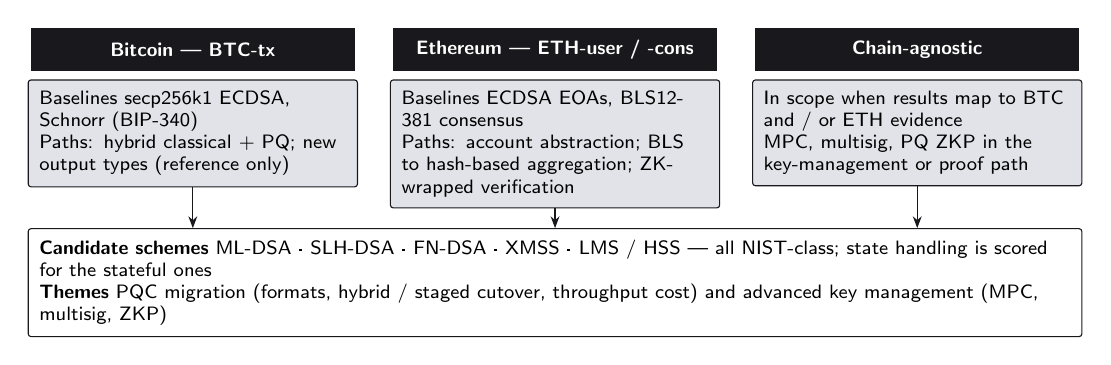
\begin{tikzpicture}[font=\scriptsize, box/.style={draw=bar,fill=lane,rounded corners=1pt,text width=3.9cm,align=left,inner sep=4pt}, hd/.style={fill=bar,text=white,font=\scriptsize\bfseries,text width=3.9cm,align=center,inner sep=3pt,minimum height=5.5mm}]
    \node[hd] (h1) at (0,0) {Bitcoin --- BTC-tx};
    \node[hd] (h2) at (4.6,0) {Ethereum --- ETH-user / -cons};
    \node[hd] (h3) at (9.2,0) {Chain-agnostic};
    \node[box,below=1mm of h1] (b1) {Baselines secp256k1 ECDSA, Schnorr (BIP-340)\\ Paths: hybrid classical + PQ; new output types (reference only)};
    \node[box,below=1mm of h2] (b2) {Baselines ECDSA EOAs, BLS12-381 consensus\\ Paths: account abstraction; BLS to hash-based aggregation; ZK-wrapped verification};
    \node[box,below=1mm of h3] (b3) {In scope when results map to BTC and / or ETH evidence\\ MPC, multisig, PQ ZKP in the key-management or proof path};
    \node[draw=bar,fill=white,rounded corners=1pt,text width=13.1cm,inner sep=4pt,align=left,below=2.5mm of b2.south,anchor=north] (ev) {\textbf{Candidate schemes} ML-DSA \textperiodcentered{} SLH-DSA \textperiodcentered{} FN-DSA \textperiodcentered{} XMSS \textperiodcentered{} LMS / HSS --- all NIST-class; state handling is scored for the stateful ones\\ \textbf{Themes} PQC migration (formats, hybrid / staged cutover, throughput cost) and advanced key management (MPC, multisig, ZKP)};
    \foreach \b in {b1,b2,b3} \draw[-{Stealth[length=1.5mm]},bar] (\b.south) -- (\b.south |- ev.north);
  \end{tikzpicture}
  \end{center}
  {\small Comparative scoring is anchored on Bitcoin and Ethereum. Every performance number is a ratio against the classical baseline on the same node, reproduced on $k$ nodes in at least two regions (gate G3).}
  \takeaway{Japan funds the prize. BGIN turns shared evidence into standards-ready artifacts. NIST remains the reference for which primitives are in scope.}
\end{frame}

%% ================================================================ discussion
\begin{frame}{Session 1-4 --- Discussion Items}
  \begin{enumerate}\small
    \item What would make a \textbf{resource estimate} usable for an evaluator --- assumptions, error bars, and what must not be collapsed into a Q-day date? What language does the rubric refuse (single Q-day, vendor screenshots)?
    \item Which \textbf{objects} move first: at-rest keys, on-spend paths, credentials, the proof and key-management path (PQ ZKP, MPC)? Open question 6 needs an owner.
    \item Is the headline quantity \textbf{total overhead} or \textbf{migration speed}? Who upgrades first, and how does M-12 record the burden split?
    \item Should the ECDSA.fail benchmark's \textbf{public-note discipline} (exact model and harness named, re-run by a validator) be the admission rule for agent-produced numbers in the record? (Decision 0001.)
    \item What does the \textbf{``PQC-ready chain'' definition} have to contain for M-22 to be scorable by December?
  \end{enumerate}
  \par\vspace{1mm}
  {\small Everything raised here is consolidated into the metric register v1 in session 1-7 at 11:30, where the scheme-scope rulings and the committee seating are taken.}
\end{frame}

% ================================================================ 15 timeline
\begin{frame}{From This Room to the 2028 Award}
  \begin{center}
  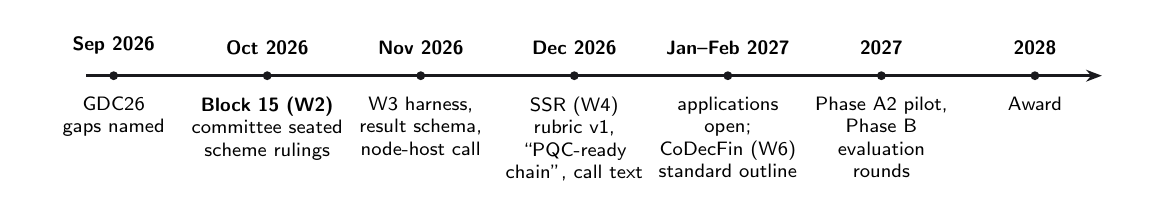
\begin{tikzpicture}[font=\scriptsize]
    \draw[line width=1pt,bar,-{Stealth[length=2mm]}] (0,0) -- (12.9,0);
    \foreach \x/\lab/\txt in {
      0.35/Sep 2026/{GDC26\\ gaps named},
      2.3/Oct 2026/{\textbf{Block 15 (W2)}\\ committee seated\\ scheme rulings},
      4.25/Nov 2026/{W3 harness,\\ result schema,\\ node-host call},
      6.2/Dec 2026/{SSR (W4)\\ rubric v1, ``PQC-ready\\ chain'', call text},
      8.15/Jan--Feb 2027/{applications open;\\ CoDecFin (W6)\\ standard outline},
      10.1/2027/{Phase A2 pilot,\\ Phase B evaluation\\ rounds},
      12.05/2028/{Award}}
      {\fill[bar] (\x,0) circle (1.6pt);
       \node[above=1.5mm,align=center,font=\scriptsize\bfseries] at (\x,0) {\lab};
       \node[below=1.5mm,align=center,text width=1.95cm] at (\x,0) {\txt};}
  \end{tikzpicture}
  \end{center}
  \par\vspace{1mm}
  \begin{center}\small
    Competition / evaluation $\rightarrow$ BGIN Standard $\rightarrow$ ISO/TC 307 $\rightarrow$ Japan's crypto-asset security criteria
  \end{center}
  {\scriptsize\color{soft} Dates are indicative until the host confirms the call. SSR 2026 PQC-for-blockchains workshop: Sun 13 Dec, Baltimore; peer-reviewed papers there are intended to be reflected in the competition specification.}
  \takeaway{This morning can still change what the call asks teams to prove. SSR on 13 December is the next drafting stop.}
\end{frame}

% ================================================================ ENGAGE
\begin{frame}{How to Engage}
  \begin{columns}[T]
    \begin{column}{0.55\textwidth}
      \begin{itemize}\small
        \item \textbf{Evaluation committee} --- draft call text, metrics and rubrics in Phase A; nominate via the issue template, with a conflict-of-interest disclosure.
        \item \textbf{Technical advisor} --- Bitcoin / Ethereum / measurement input without winner votes.
        \item \textbf{Metric or scheme proposal} --- an issue, then a pull request to the register. Every commit is signed and signed-off; a PR is the record.
        \item \textbf{SSR workshop, 13 Dec} --- accepted papers feed the competition specification.
        \item \textbf{Next}: session 1-7 at 11:30, same room --- agility as a governance property, the NIST path, the W2 decisions.
      \end{itemize}
    \end{column}
    \begin{column}{0.42\textwidth}
      \begin{center}\tiny
        \begin{tabular}{@{}>{\centering\arraybackslash}p{1.85cm}@{\hspace{1mm}}>{\centering\arraybackslash}p{1.85cm}@{\hspace{1mm}}>{\centering\arraybackslash}p{1.85cm}@{}}
          \qrcode[height=1.35cm]{https://bgin-global.org/events/20261015-block15/sessions/1-4} &
          \qrcode[height=1.35cm]{https://github.com/bgin-global/pqc-agility-competition} &
          \qrcode[height=1.35cm]{https://bgin.discourse.group/c/post-quantum-crypto-agility-competition/44} \\[0.5mm]
          \textbf{This session} & \textbf{Repository} & \textbf{Discourse category} \\
          bgin-global.org/events/ 20261015-block15/sessions/1-4 & github.com/bgin-global/ pqc-agility-competition & bgin.discourse.group/c/ post-quantum-crypto-agility-competition/44
        \end{tabular}
      \end{center}
    \end{column}
  \end{columns}
  \takeaway{Discussion on Discourse; the repository is the record. Nothing is final until the committee ratifies it and the host publishes the call.}
\end{frame}

% ================================================================ CLOSE
{\setbeamertemplate{footline}{}
\begin{frame}[plain]
  \begin{tikzpicture}[remember picture,overlay]
    \fill[bar] (current page.north west) rectangle (current page.south east);
    \node[anchor=south,text=white,font=\Large\bfseries,text width=13.5cm,align=center,execute at begin node=\nohyph] at ([yshift=6mm]current page.center){An estimate enters the rubric as a declared assumption with error bars --- never as a date.};
    \node[anchor=north,text=white,font=\small,text width=13.5cm,align=center,execute at begin node=\nohyph] at ([yshift=3mm]current page.center){The hard problem is deployment, evaluation, and migration governance. Not selecting a new primitive. Not a Q-day. Not an endorsement.};
    \node[anchor=north,text=soft,font=\small,text width=13.5cm,align=center,execute at begin node=\nohyph] at ([yshift=-9mm]current page.center){BGIN IKP Working Group \textperiodcentered{} Post-Quantum Crypto Agility Competition category on the BGIN Discourse \textperiodcentered{} github.com/bgin-global/pqc-agility-competition};
    \node[anchor=south east,inner sep=0] at ([xshift=-7mm,yshift=5mm]current page.south east){
\includegraphics[height=1.4cm]{bgin_logo.png}};
  \end{tikzpicture}
\end{frame}}

\end{document}
